\documentclass[14pt]{beamer}
\usetheme{Antibes}
\definecolor{myOrange}{RGB}{238,97,53}
\setbeamercolor*{palette primary}{fg=myOrange}
\setbeamercolor*{palette secondary}{fg=myOrange,bg=white}
\setbeamercolor*{palette tertiary}{bg=myOrange,fg=white}
\setbeamercolor*{titlelike}{parent=palette primary}
\setbeamercolor*{itemize item}{fg=myOrange}
\setbeamercolor{block title example}{bg=myOrange} 
\setbeamercolor{section in toc}{fg=black}
\setbeamertemplate{sections/subsections in toc}[sections numbered]
\setbeamercolor{section number projected}{bg=myOrange,fg=yellow}
\setbeamertemplate{footline}[frame number]
\setbeamertemplate{frametitle}{
  \begin{centering}
  \insertframetitle
    \par
    \end{centering}
}
\setbeamertemplate{itemize item}{\textbullet}

\usepackage{amsmath}
\usepackage[english]{babel}
\usepackage{listings}
\usepackage{hyperref}
\logo{
\includegraphics[width=1cm]{logo.png}}
\newcommand\B{\rule[-1.7ex]{0pt}{0pt}}

\setcounter{tocdepth}{1}

\begin{document}
\title{RegExp in Java, TOS and IntelliJ}
\author{Arkady Galyash}
\institute{TosChart}
\date{\today}

\newcommand{\smaller}[1] {
  {\scriptsize {#1}}
}

% Здравствуйте, меня зовут Аркадий Галяш, я работаю в команде тосчарт. 
% Сегодня я представляю вашему вниманию презентацию на тему "Регулярные выражения в Джава, Тосе и Интеллиджи",
% Вопросы можно задавать как походу доклада, так и в конце.
\frame{\titlepage}


% Сначала мы кратко вспомним, насколько разные вещи мы называем одним и тем же словосочетанием регулярные вырадения, зачем их знать и какова их область применения
% Потом рассмотрим как реализована поддержка регулярных выражений в Джава, а так же какие ограничения и потенциальные ошибки вызывает данная реализация.
% Сразу после этого мы рассмотрим различные "странности", которые я заметил, рассмотрев код тоса и тосчарта.
% И в конце доклада мы рассмотрим как поддерживается работа с регулярными выражениями в Интеллидж, а также как улучшить эту поддержку, как написать свои инспекции для идеи и прочие подобные вопросы 
\frame%
{\frametitle{Agenda}
  \tableofcontents[1]
}

% Сначала хочется посмотреть как менялось понятие регулярных выражение сквозь года и назвать тех людей, которые внесли большой вклад в развитие и популяризацию регулярных выражений,
% Первым хочется упомянуть Стивена Клини(американского профессора) Именно он в 50ые годы предложил символы для описания замыканий, поэтому часто их называют звезда Клини, плюс Клини,
% Следующая эпоха связана с операционной системой юникс и лично Кеном Томпсоном. До начала 70х годов регулярные языки были лишь забавным подмножеством и были известны лишь в академической среде, До тех пор пока Кен Томпсон не прочитал научную статью о регулярных языках и обнаружил их огромную потенциальную пользу для обработки текста.
% Поэтому поддержка регулярных выражений была встроена в редактор ед, а потом и во все остальные утилиты по работе с текстом. Хочется заметить, что это были именно регулярные выражения в классическом понимании(соотвествующие решулярным языкам и реализованный при помощи детерменированного конечного автомата)
% Дальнейшее развитие регулярные выражения получили в 88 году, когда Ларри Уолл выпустил 2 версию своего языка Перл. И после этого мир регулярных выражений никогда не станет прежним. Кроме различных косметических улучшений и изменений, была расширена и выразительная мощность регулярных выражений
% При помощи регулярных выражений Перла можно например описать язык корректной скобочной записи, который как известно не является автоматным(регулярным). Как следствие, Перловые регулярные выражения уже не могут быть реализованы при помощи построения детерменированного конечного автомата - они используют недетерминированный.
% Существуют различные точки зрения на Перловые регулярные выражения. Но точно можно сказать, что все эти расширения понравились такому большому количеству людей, что их поддержка была добавлена в GNU имплементации классических утилит 70х годов (например, grep)
% Да и вообще на данный момент, большинство программ поддерживают перловую интерпретацию регулярных выражений.
\section{RegExp in Java}
\subsection{History}
\frame{\frametitle{History}
  \begin{itemize}
    \item Before UNIX(Stephen Cole Kleene, 1950s): automata theory
    \item UNIX(Ken Thompson, 1970s): QED, ed, g/re/p, ...
    \item Perl(Larry Wall, 1988): 2nd edition
  \end{itemize}
}

% А почему вообще регулярные выражения так важны и зачем программисту хорошо бы уметь ими пользоваться?
% Во-первых, регулярные выражения - это тот "багаж", который всегда с Вами. Один раз научившись пользоваться регулярными выражениями - вы сможете применять их повсеместно.
% Многие языки программирования/библиотеки/инструменты умерли/вышли из моды/перестали использоваться, а регулярные выражения с 70х годов и до сих являются мейнстримом и важным и полезным ноухау.
% Практически все разрабатываемые вами серьезные программы, скорее всего, логгируют свои действия, анализ этих логфайлов можно существенно упростить, используя регулярные выражения.
% Так же регулярные выражения можно по прежнему использовать для той самой первой задачи, для которой они были впервые применены - редактирование текста. Если ваш текстовый редактор сложнее блокнота - то готов поспорить, что он поддерживает поиск и замену с поддержкой регулярных выражений.
% Еще регулярные выражения обычно применяются при написании лексических анализаторов(например утилиты lex и ее производные)
% Ок, предположим, что вы не пишете лексеры, не читаете логи и у вас хитрая иде, в которой можно обойтись без использования трегулярных выражений.
% Но если вы разрабатываете клиентское приложение, то очень вероятно, что вам нужно проверять на корректность ввод пользователя - и тут опять на помощь вам опять придут регулярные выражения
% Если я до сих пор вас не убедил, что регулярные выражения знать важно и полезно. В качестве предпоследнего аргумента могу сказать, что лично для меня - это знание, которое я применяю каждый день чаще всего. 
\subsection{Why developer should know RegExp?}
\frame{\frametitle{Why developer should know RegExp?}
  \begin{itemize}
    \item Learn once, use anywhere
    \item Extract needed info from log files(grep)
    \item Advanced text editing
    \item Using lexer generators(lex) and syntax highlighting
    \item ...
  \end{itemize}
}

% В качестве же совсем последнего аргумента - хочется заметить, что регулярные выражения сделают вас этаким супергероем в глазах непосвещенных, кто не овладел ими в полной мере, потому что вы с легкостью будете выполнять и автоматизировать различные внешне сложные задачи.
% Ну и конечно доклад про регулярные выражения не мог обойтись без соответсвующего комикса xkxd
\frame{\frametitle{Do you want to be a Superhero?}
  \begin{center}
    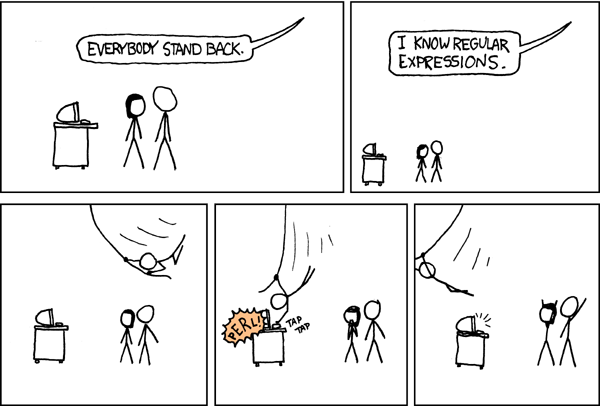
\includegraphics[height=0.8\textheight]{xkcd2.png}
  \end{center}
}

% Однако за кажущейся простотой регулярных выражений скрывается огромная мощь и сила. А как мы знаем, с большой силой приходит большая ответсвенность. 
% Вершиной мастерства использования регулярных выражений, как мне кажется, является не умение использовать их, когда надо, а умение не использовать их, когда не надо.
\begin{frame}
\begin{exampleblock}{}
  {\large With great power there must also come — great responsibility!}
    \vskip3mm
    \hspace*\fill{\small--- Stan Lee, ``Spider-Man''}
\end{exampleblock}
\begin{exampleblock}{}
  {\large Some people, when confronted with a problem, think "I know, I'll use regular expressions."  Now they have two problems.}
    \vskip3mm
    \hspace*\fill{\small--- Jamie Zawinski, alt.religion.emacs}
\end{exampleblock}
\end{frame}

% Обратимся теперь к особенностям реализации движка регулярных выражений в языке джава и обсудим как те или иные решения повлияли на удобство использования регулярных выражений в джава.
% Как всем присутсвующим, наверно, известно, в джава движок регулярных выражений сделан по образу и подобию перлового с небольшими косметическими расширениями и ограничениями. 
% Кроме того, в отличии от перла регулярные выражения не встроены в язык, а являются отдельной библиотекой, которая умеет компилировать простые строки языка джава в соотвествующие конечные автоматы для распознования и работы с регулярными выражениями
% Одной из фич перловой поддержки регулярных выражений, которой лично мне активно не хватает в джава это прекомпилированные регулярные выражения(qr). 
% В реальной жизни я видел решения проблемы с переиспользованием отдельных кусков регулярных выражений в джаве при помощи конкатенации строк. Но мне кажется, что это не очень удачное решение, ибо в отличии от qr интерпретация регулярного выражения зависит от того, что стоит перед ним, что затрудняет его анализ и понимание. Далее у меня будет реальный наглядный пример из жизни
% Ну и конечно нельзя не упомянуть этот ад обратных косых черт в который превращается работа с регулярными выражениями в джава, т.к. строковые литералы языка джава требуют ставить двойную косую черту, которая имеет особое значение внутри  регулярных выражений.
\frame{\frametitle{RegExp in Java}
  \begin{itemize}
    \item simple strings, compiled by java.util.regex.Pattern
    \item no qr//, concatination of strings is really bad idea
    \item ``backslashes hell''
  \end{itemize}
}

\def\colored#1{\textcolor{myOrange}{#1}}
\def\^{\char94}
\def\doubleslash{\textbackslash\textbackslash}

\def\regexphow #1#2#3#4{
  \subsection{#2}%
  \begin{frame}[t]%
  \frametitle{RegExp HowTo \##1}%
  $ $ \\%
  \begin{tabular} {p{2cm} @{}p{8cm}}%
    \colored{Task:} \B & #2\\% \pause\\%
    \colored{Cases:} \B%
%      \onslide<2->%
        & \large \ttfamily #3%
%    \onslide*<3->%
     \\ \colored{Prefer:} \B & \large \ttfamily #4%
  \end{tabular}%
  \end{frame}%
}%

\def\regexpexample #1#2#3#4#5#6{
  \subsection{#2}%
  \begin{frame}[t]%
  \frametitle{RegExp \##1}%
  $ $ \\%
  \begin{tabular} {p{2cm} @{}p{8cm}}%
    \colored{Task:} \B & #2\\% \pause\\%
    \colored{Case:} \B%
%      \only<2>%
%        {& \large \ttfamily #3}%
%      \onslide*<3->%
        & \large \ttfamily #4%
%    \onslide*<4->%
     \\ \colored{Fix:} \B & \large \ttfamily #5%
%    \onslide*<5->%
     \\ \colored{Rule:} \B & #6%
  \end{tabular}%
  \end{frame}%
}%

% т.к. я смотрю многие уже успели соскучиться и медленно впадают в кому, поэтому вторая часть моего доклада будет более-менее активной и игровой. Сейчас я буду показывать реальные регулярные выражения из проектов тос и тосчарт, которые вызвали у меня те или иные вопросы(подчеркиваю, не оказались совсем не правильными, а вызвали вопросы)
% Потом надеюсь аудитория угадает, что именно меня смутило и как сделать этот паттерн не таким смущяющим
% В конце слайда, обсуждение, так что если  у кого-то будут какие-то замечания/идеи/возражения, то это идеальное место, чтобы их озвучить
\section{RegExp in TOS}
\frame{\frametitle{RegExp CodeStyle in TOS}
  \begin{itemize}
    \item Real task.
    \item Used solution(case).
    \item Guess what's wrong with this case codestyle?
    \item Thoughts about this case and how to avoid wrong patterns.
    \item Discussion.
  \end{itemize}
}

% Итак, первый пример: текст внутри фигурных скобок.
% Вот такое решение предложил программист. Что в нем смущает? Правильно, экранирование закрывающей скобки внутри класса символов
% Важно помнить, что внутри и снаружи классов различные символы имеют особое значение и должны соответсвенно должны экранироваться
\subsection{Strange RegExps}
\regexpexample{1}{text inside \{\}}
  {(\doubleslash{}\{([\^\doubleslash{}\}]*)\doubleslash{}\})}
  {(\doubleslash{}\{([\^\colored{\doubleslash{}\}}]*)\doubleslash{}\})}
  {(\doubleslash{}\{([\^\}]*)\doubleslash{}\})}
  {Do not escape characters that do not need escaping inside character classes}

% Следующий пример: произвольное количество пробельных символов(пробелов, табуляций, переводов каретки, новых строк и т.д.)
% В одном из регулярных выражений в тосе использовалась следующая запись. Есть у кого-нить идеи что с ней не так? 
% Правильно, простая группа символов \s уже содержит в себе перевод каретки и символ новой строки.
% Кроме того, что такая запись бессмысленна, она еще и работает медленнее.
% Соответсвенно, важно помнить, что скрывается за простыми группами символов(благо, что их не так много). А так же помнить, что они работают как внутри, так и вне классов символов
\regexpexample{2}{match whitespace characters(blank, CR, NL, TAB, etc.)}
  {[\doubleslash{}s\textbackslash{}r\textbackslash{}n]*}
  {[\doubleslash{}s\colored{\textbackslash{}r\textbackslash{}n}]*}
  {[\doubleslash{}s]*}
  {Remove from character classes single chars that are already there}

% Третий пример - это пробельные символы заканчивающиеся точкой с запятой.
% Решение из тосчарта, работает и работает правильно, но выглядит странно и не привычно моему, к примеру, глазу. Что же меня смущает?
% Правильно, эти абсолютно не несущие никакой смысловой нагрузки скобки классов символов.
% Их можно спокойно опустить без потери смысла, все что они делают просто занимают место.
\regexpexample{3}{semicolon with leading whitespaces}
  {[\doubleslash s]*[;]}
  {\colored{[}\doubleslash{}s\colored{]}*\colored{[};\colored{]}}
  {\doubleslash{}s*;}
  {Remove character classes when they are unneeded}

% Этот пример мы будем последовательно улучшать на 2х слайдах подряд. Тут мне уже проблематично было выделить маленькую часть.
% Итак, что с ним не так? Первое, что цепляет глаз - это выставленная опция "игнорирования регистра" для регулярного выражения без букв.
% В реальном примере, там как раз это регулярное выражение было частью другого и в последуюших состовляющих буквы как раз были.
% Это как мне кажется, хороший пример, что использовать конкатенацию строк для регулярных выражений из-за подобных побочных эффкетов - не самая хорошая идея.
% Во-первых, если вдруг опция действительно не на что не влияет, то лучше ее и не писать.

\regexpexample{4}{part of complex regexp}
  {(?i)(([\doubleslash{}n\doubleslash{}r]+)|(\^))}
  {\colored{(?i)}(([\doubleslash{}n\doubleslash{}r]+)|(\^))}
  {(([\doubleslash{}n\doubleslash{}r]+)|(\^))}
  {Remove useless inline modifiers}

% Во-вторых, хочется заметить, что если вы хотите включить опцию глобально, то не обязательно писать ее в начале. В классе Pattern кроме известного вам метода compile есть его расширенная версия с 2мя параметрами. 
% Во второй параметр можно передать набор опций, которые вы хотите включить глобально.
\begin{frame}[fragile]
\frametitle{java.util.regex.Pattern\#compile(...)}
  \begin{lstlisting}[language=Java, frame=single, basicstyle=\small, stringstyle=\color{myOrange}]
String A = "(?i)\s*";
String B = "test";
...
Pattern p = Pattern.compile(A + B);
  \end{lstlisting}
  \begin{center}VS\end{center}
  \begin{lstlisting}[language=Java, frame=single, basicstyle=\small, stringstyle=\color{myOrange}]
String A = "\s*";
String B = "test";
...
Pattern p = Pattern.compile(A + B,
              Pattern.CASE_INSENSITIVE);
  \end{lstlisting}
\end{frame}
% Итак из исходного регулярного выражения мы удалили включение не нужной опции, что еще в нем можно улучшить?
% Правильно, захват так называемого ассершена нулевой длины. Он бессмысленен, т.к. эта группа всегда вернет вам пустую строку
% Убрав и ненужные скобки вокруг сивола начала строки, получим уже вполне читабельное регулярное выражение
\regexpexample{5}{part of complex regexp \#2}
  {(([\textbackslash{}n\textbackslash{}r]+)|(\^))}
  {(([\textbackslash{}n\textbackslash{}r]+)|\colored{(\^)})}
  {(([\textbackslash{}n\textbackslash{}r]+)|\^)}
  {Remove useless capturing(for zero-width assertions)}

% Последний пример это просто большой кусок текста внутри регулярного выражения
% Что тут не так? Правильно, все эти слеши для экранирования спец-символов мешают нам читать текст, слава богу, в регулярных выражениях есть замечательная фича - автоматическое экранирование
% Соответственно, я считаю, что в данном конкретном случае его использование вполне оправдано и сделает регулярное выражение более читабельным
\regexpexample{6}{copyright}
  {\doubleslash{}(company\doubleslash{}. \doubleslash{}(c\doubleslash{})\doubleslash{})}
  {\colored{\doubleslash{}(company\doubleslash{}. \doubleslash{}(c\doubleslash{})\doubleslash{})}}
  {\doubleslash{}Q(company. (c))\doubleslash{}E}
  {Use \textbackslash{}Q...\textbackslash{}E when it is appropriate}

% Следующие 4 слайда содержат не столько подозрительные куски регулярных выражений, сколько не стандартизированные вопросы стиля
% Например, частенько можно встретить запись !произвольная цыфра! не через простой класс символов. Лично я считаю, что второй вариант предпочтительней.
\subsection{RegExp CodeStyle}
\regexphow{1}{digit}
  {[0-9] or \doubleslash{}d}
  {\doubleslash{}d}

% Не знаю, откуда взялся первый паттерн с этого слайда - это пример того, как иногда легко становятся популярными странные и не очевидные решения
% В регулярных выражениях есть спец опция включение/выключение которой меняет поведение точки(матчит она или нет символы перевода каретки и конца строки)
% Но вместо ее люди часто используют 2 противоположных простых класса символов, что не только медленнее работает, но и контр-интуитивно, а к тому же занимает больше места
\regexphow{2}{any symbol(including NL, CR, etc.)}
  {[\doubleslash{}w\doubleslash{}W] or (?s:.)}
  {(?s:.)}

% Вопрос как же именно экранировать символы имеющие спец значения так же остается открытым
% Тут у меня нет определенного мнения, но наверно подсознательно мне хочется избежать ада обратных слешей
\regexphow{3}{How to escape special chars?}
  {[.] or \doubleslash{}.}
  {[.]}

% Последний интересный вопрос как же писать символы табуляции, конца строки и перевода каретки?
% Их можно писать с одним или двумя слешами: это потому что один слеш "сдирается" компилятором джава. Т.е. в случае с одним слешом компилятору паттернов отдается сразу символ с кодом 13, например. В случае же двух слешей компилятору паттернов отдается последовательность обратный слеш + буква n, которую он трактует как новую строку.
% Здесь я настоятельно рекомендую использвать ВСЕГДА один слеш: в бессильной попытке как-то упорядочить ад обратных слешей.
% Просто тогда: видишь один слеш - это символ, видишь 2 - простой класс символов, 4 - слеш.
\regexphow{4}{CR, Tab, NL}
  {\doubleslash{}n or \textbackslash{}n}
  {\textbackslash{}n}

% Вот мы с вами поговорили полчаса, обсудили и согласились, что надо писать хорошие регулярные выражения и не надо писать плохие. Но стоит нам всем разойтись по рабочим местам и рутина затянет нас и вы уже через час даже не вспомните, о чем мы тут с вами разговаривали.
% Поэтому я написал инспекции для идеи, реализующие все описанные аспекты, отраженные в презентации. На случай, если кто-то разделяет мою точку зрения и хочет поддержки иде в данном вопросе.
% Мой прошлый доклад был раскритикован за отсутствие подробностей как писать свои плагины для идеи, поэтому в этот я добавил соответствующую секцию в этот.
% Сначала числовые характеристики: 10 инспекции(классических, работают в коммон-едишн), написал за пару выходных, где-то 2 тыщи строк кода(включая юнит-тесты)
% Правда, нужно понимать, что я встал на плечи гигантов - просто парсер и внутреннее представление для регулярных выражений уже были написаны, за что огромное спасибо автору.
% Так что мое - это только сами инспекции.
\section{RegExp in IntelliJ}
\subsection{RegExp inspections}
\frame{\frametitle{RegExp inspections}
  \begin{itemize}
    \item 10 inspections(old-fashion, work in CE too)
    \item 2 weekends
    \item 2000 LOC in 25 *.java files(including unit tests)
    \item A lot of kudos to Sascha Weinreuter(language injection plugin)
  \end{itemize}
}

% Установить этот набор инспекций можно прямо из идеи, называется он RegExpNazi.
% Если вдруг, что-то с ним не так, он у вас не заработал или заработал не так как вы ожидали - пишите мне письма/багрепорты - разберемся.
% Если вам вдруг понадобиться код или вы починили какую-то багу и т.д. - все лежит на гитхабе - пишите.
\subsection{RegExpNazi}
\frame{\frametitle{RegExpNazi}
  \begin{center}
    
\includegraphics[width=0.5\textwidth]{optocat.png}  \\
    \large \href{https://github.com/gark87/RegExpNazi}{https://github.com/gark87/RegExpNazi}
  \end{center}
}

% Итак, что же делать, если хочется написать свой набор инспекций? Как и для всех других случаях когда вам нужен плагин для идеи - первое с чего нужно начать - описание нужных точек расгирения в файле plugin.xml
% Нужная нам называется - inspectionToolProvider. там мы указываем имя класса - провайдера списка добавляемых нами инспекций
\subsection{How to write our inspections set?}
\frame{\frametitle{Start}
  \begin{itemize}
    \item package com.intellij.codeInspection
    \item plugin.xml:\\
      {\small$<$inspectionToolProvider implementation="..."$>$}
    \item interface InspectionToolProvider\\
           implement Class[] \#getInspectionClasses()
    \item LocalInspectionTool
  \end{itemize}
}

% итак а что же представляет из себя одна инспекция? Она проверяет файл и выдает массив описаний найденных ошибок. Кроме того, есть еще 3 обязательных метода, которые вы должны определить
% первыe 2 отвечает за то, какое имя(название) будет отображены в списке инспекции и как называется группа, которой эта инспекция пренадлежит
% третья - это имя HTML файла с описанием этой инспекции.
% Если ваша инспекция имеет какие-либо настраиваемые параметры, то можно переопределить метод createOptionsPanel и возвращать компонент для настроики этих самых параметров.
% Сами настройки хранить следует в качестве публичных полей инспекции
\frame{\frametitle{LocalInspectionTool}
  \begin{itemize}
    \item ProblemDescriptor[] \#checkFile(...)\\
    check only our filetypes
    \item String \#getGroupDisplayName()\\
    String \#getDisplayName()
    \item String \#getShortName() \\
    HTML file with help
    \item JComponent \#createOptionsPanel()\\
    use public fields to store options
  \end{itemize}
}

% Еще немного разных подробностей: лично мне кажется, что инспекция без предложения автоматического исправления - не совсем честно, поэтому все мои инспекции умеют чинить себя сами.
% Для этого необходимо создать подкласс LocalQuickFix и определить в нем метод applyFix, который и будет делать всю важную часть работы, а именно модифицировать внутреннее представление соотвествующим образом
% Если замена это достаточно сложное и расвесистое поддерево, иногда бывает проще просто создать виртуальный файл записать в него текстовое представление этого дерева, распарсить и использовать полученный результат.
% Написание юнит-тестов для интеллидж - одна из самых неблагодарных задач, очень не удобно, не документировано и неприятно.
% Сложно - но можно. Правда, весь их тестовый фреймворк заточен под работу с файлами, так что будьте готовы, что в конечном итоге все равно ваши тесты так или иначе будут работать именно с файлами, даже если вам нужно распарсить строку из 10 символов.
% Кроме того, есть некий набор ритуальных заклинаний, которые можно найти только на форумах и т.д. Так что настоятельно рекомундую, лучше взять тесты из плагина наиболее близкого вашему по духу и модифицировать их под свои нужды.
\frame{\frametitle{Miscellaneous}
  \begin{itemize}
    \item LocalQuickFix 
      \begin{itemize}
        \item \#applyFix()
        \item fix AST and PSI trees properly
        \item if replacement is really hard to construct then you can use fake file
      \end{itemize}
    \item Unit tests
      \begin{itemize}
        \item file-based
	\item -Didea.platform.prefix="Idea"
      \end{itemize}
  \end{itemize}
}

% Ссылки 
\section{Links}
\frame{\frametitle{Links}
  \begin{itemize}
    \item \href{https://www.coursera.org/\#course/automata}{coursera.org course by Jeffrey Ullman}
    \item \href{http://swtch.com/~rsc/regexp/regexp1.html}{Regular Expression Matching Can Be Simple And Fast(but is slow in Java, Perl, PHP, Python, Ruby, ...) by Russ Cox}
    \item ``Mastering Regular Expressions'' by Jeffrey Friedl
    \item \href{https://twitter.com/\#!/RegexTip}{@RegexTip}
    \item man perlre*
  \end{itemize}
}
\frame{
  \begin{center}
    Thank You!
  \end{center}
}

\end{document}
